\section{Resistencia eléctrica}
Es la oposición que recibe el electrón en su desplazamiento a través de un conductor. Su unidad de medida en el sistema internacional es el ohmio y que es representa con la letra griega omega (\textohm). Fue descubierto en 1827 por el físico alemán Greog Ohm, y a honor su apellido es la  unidad de medida.

\begin{equation*} 
	R = \rho\dfrac{\ell}{S}\\	
\end{equation*}
Donde:\\
$ \rho $: es el coeficiente de proporcionalidad o la resistividad del material.\\
$\ell$: es la longitud del alambre.\\
$S$: es el área de la sección transversal del alambre.\\
Para que su valor sea medido se  una la herramienta de medición llamada ohmnímetro. La otra manera de ser medido es un circuito, la resistencia es directamente proporcional al voltaje y inversamente proporcional a la corriente eléctrica que circula en el circuito. En  la siguiente ecuación podremos observar con mas precisión lo mencionado:
\begin{equation*}
	R=\dfrac{V}{I}
\end{equation*}
Donde:\\
$ R $: es la resistencia (\textohm).\\
$ V $: es el voltaje ($V$).\\
$I$: es la intensidad de corriente ($A$).\\
\section{Asociación de resistencias}
Consiste en encontrar el valor equivalente de las resistencias en un circuito. Las resistencias se pueden encontrar asociadas en serie o paralelo, de tal manera que se pueda tener una resistencia equivalente para todo ello.
\subsection{Asociación en serie}
La asociación en serie, es cuando las resistencias están conectadas entre si una a continuación de  otra como se muestra en la figura 1:\\
\begin{figure}[h]
	\centering
	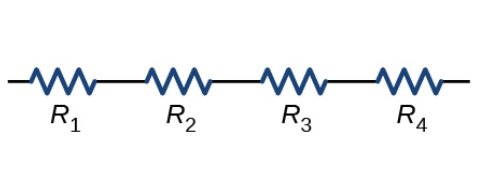
\includegraphics{imagenes/serie}
	\caption{Circuito en serie}
\end{figure}\\
En este tipo de circuitos la intensidad de corriente es la misma para todas las resistencias, mientras el voltaje varia en cada una de las resistencias de acuerdo a la capacidad que tienen. La ecuación para hallar la resistencia equivalente es la siguiente:
\begin{equation*}
	R_{eq}= R_{1} + R_{2}+ R_{3} + .....  + R_{n}
\end{equation*}
\subsection{Asociación en paralelo}
La asociación en paralelo, es cuando sus terminales en común están conectadas a un mismo punto del circuito como se muestra en la figura 2:\\
\begin{figure}[h]
	\centering
	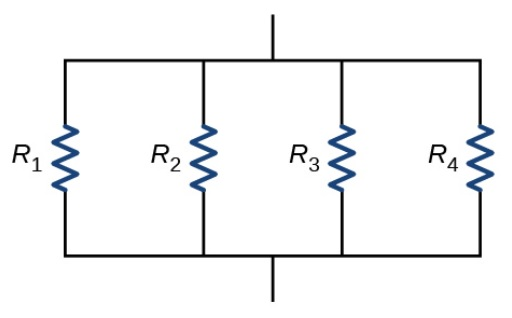
\includegraphics{imagenes/paralelo}
	\caption{Circuito en paralelo}
\end{figure}\\
En este tipo de circuitos el voltaje que circula será lo mismo para cualquiera de las resistencias, mientras tanto la intensidad de corriente varia en cada una de las resistencias de acuerdo a su resistividad. La ecuación para hallar la resistencia equivalente es la siguiente:
\begin{equation*}
	\dfrac{1}{R_{eq}} = \dfrac{1}{R_{1}} + \dfrac{1}{R_{2}} + \dfrac{1}{R_{3}} + ..... + \dfrac{1}{R_{n}}
\end{equation*}
\section{Código de colores en resistencias}
En el mundo electrónico podemos encontrar muchas variedades de resistencias, y también diversos métodos para calcular sus valores reales. Uno de estos métodos es el código de colores,  que están definidos en las normas internacionales de la IEC 60062. Estos estándares son universales y únicos en el mundo.\\
Hay varias bandas para especificar el valor de la resistencia. Incluso especifican tolerancia, confiabilidad y tasa de fallas. El número de bandas varía de tres a seis. En el caso del código de 3 bandas, las dos primeras indican el valor de la resistencia y la tercera banda actúa como multiplicador.\\
Veamos las siguientes figuras para reconocer y diferenciar las variedades de resistencias.\\
\begin{figure}[h]
	\centering 
	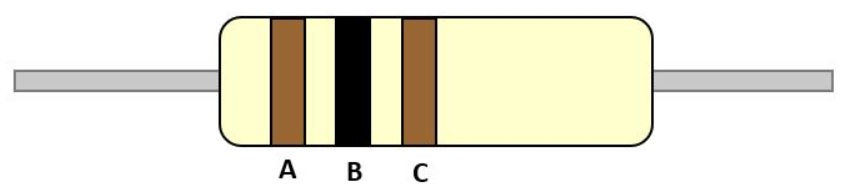
\includegraphics[width=15cm]{imagenes/tresbandas}
	\caption{Resistencia de tres bandas}
\end{figure}\\
Para poder calcular su valor tenemos que reemplazar los valores de los colores en la siguiente ecuación:\\
\begin{equation*}
	ABxC \pm 20\%
\end{equation*}\\
Donde: \\
$ A $: 1° banda es la primera cifra significativa.\\
$ B $: 2° banda es la segunda cifra significativa.\\
$ C $: 3° banda es el multiplicador.\\

\begin{table}[h]
	\begin{center}
		\begin{tabular}{|c | c | c | c |}
			\hline
			Color& 1° banda & 2° banda & Multiplicador \\
			 \hline
			Negro&& 0 &$ 10^{0}$ \\
			\hline
			Marrón & 1&1&$ 10^{1}$\\
			\hline
			Rojo & 2&2&$ 10^{2}$\\
			\hline
			Naranja & 3&3&$ 10^{3}$\\
			\hline
			Amarillo & 4&4&$ 10^{4}$\\
			\hline
			Verde & 5&5&$ 10^{5}$\\
			\hline
			Azul & 6&6&$ 10^{6}$\\
			\hline
			Violeta & 7&7&$ 10^{7}$\\
			\hline
			Gris & 8&8&$ 10^{8}$\\
			\hline
			Blanco & 9&9&$ 10^{9}$\\
			\hline
		\end{tabular}
		\caption{Código de colores para resistencias de tres bandas.}
	\end{center}
\end{table}
\begin{figure}[h]
	\centering 
	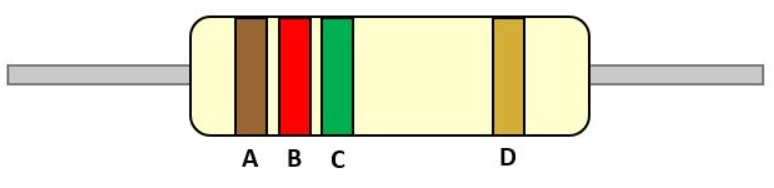
\includegraphics[width=15cm]{imagenes/cuatrobandas}
	\caption{Resistencia de cuatro bandas}
\end{figure}
Para poder calcular su valor tenemos que reemplazar los valores de los colores en la siguiente ecuación:\\
\begin{equation*}
	ABxC \pm D\%
\end{equation*}\\
Donde: \\
$ A $: 1° banda es la primera cifra significativa.\\
$ B $: 2° banda es la segunda cifra significativa.\\
$ C $: 3° banda es el multiplicador.\\
$D$: 4° banda es la tolerancia que tiene la resistencia.\\
\\
\\
\begin{table}[h]
	\begin{center}
		\begin{tabular}{|c | c | c | c |c|}
			\hline
			Color& 1° banda & 2° banda & Multiplicador & Tolerancia $ \% $\\
			\hline
			Negro& & 0 &$ 10^{0}$ & 0\\
			\hline
			Marrón & 1&1&$ 10^{1}$&1\\
			\hline
			Rojo & 2&2&$ 10^{2}$&2\\
			\hline
			Naranja & 3&3&$ 10^{3}$&3\\
			\hline
			Amarillo & 4&4&$ 10^{4}$&4\\
			\hline
			Verde & 5&5&$ 10^{5}$&0.5\\
			\hline
			Azul & 6&6&$ 10^{6}$&0.25\\
			\hline
			Violeta & 7&7&$ 10^{7}$&0.1\\
			\hline
			Gris & 8&8&$ 10^{8}$&0.05\\
			\hline
			Blanco & 9&9&$ 10^{9}$&\\
			\hline
			Oro & &&$ 10^{-1}$&5\\
			\hline
			Plata & &&$ 10^{-2}$&10\\
			\hline
		\end{tabular}
		\caption{Código de colores para resistencias de cuatro bandas.}
	\end{center}
\end{table}

\begin{figure}[h]
	\centering 
	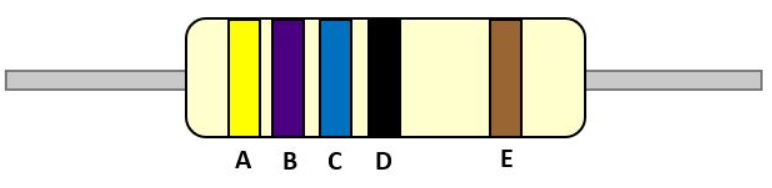
\includegraphics[width=15cm]{imagenes/cincobandas}
	\caption{Resistencia de cinco bandas}
\end{figure}

Para poder calcular su valor tenemos que reemplazar los valores de los colores en la siguiente ecuación:\\
\begin{equation*}
	ABCxD \pm E\%
\end{equation*}\\
Donde: \\
$ A $: 1° banda es la primera cifra significativa.\\
$ B $: 2° banda es la segunda cifra significativa.\\
$ C $: 3° banda es la segunda cifra significativa.\\
$ D $: 4° banda es el multiplicador.\\
$E$: 5° banda es la tolerancia que tiene la resistencia.\\
\\
\\
\\
\\
\\
\\
\\
\\
\\
\\
\\
\begin{table}[h]
	\begin{center}
		\begin{tabular}{|c | c | c | c |c|c|}
			\hline
			Color& 1° banda & 2° banda &3°banda& Multiplicador & Tolerancia $ \% $\\
			\hline
			Negro&&0 & 0 &$ 10^{0}$ & 0\\
			\hline
			Marrón &1& 1&1&$ 10^{1}$&1\\
			\hline
			Rojo & 2&2&2&$ 10^{2}$&2\\
			\hline
			Naranja & 3&3&3&$ 10^{3}$&3\\
			\hline
			Amarillo & 4&4&4&$ 10^{4}$&4\\
			\hline
			Verde & 5&5&5&$ 10^{5}$&0.5\\
			\hline
			Azul & 6&6&6&$ 10^{6}$&0.25\\
			\hline
			Violeta & 7&7&7&$ 10^{7}$&0.1\\
			\hline
			Gris & 8&8&8&$ 10^{8}$&0.05\\
			\hline
			Blanco & 9&9&9&$ 10^{9}$&\\
			\hline
			Oro && &&$ 10^{-1}$&5\\
			\hline
			Plata && &&$ 10^{-2}$&10\\
			\hline
		\end{tabular}
		\caption{Código de colores para resistencias de cinco bandas.}
	\end{center}
\end{table}

Como se pudo observar para cada tipo de resistencia existe un código respectivo, que varia dependiendo el número de bandas o franjas que posee una resistencias. Por lo tanto para hallar el valor de una resistencia mediante el uso del código de colores, es necesario tener una tabla de equivalencias al momento de la búsqueda del valor real de una resistencia.